\chapter{Architectural Design}
We have decided to build \textbf{\textit{Flats}} using Flutter. Flutter is an open source framework developed by Google for building natively compiled and multi-platform applications from a single codebase. Flutter is powered by Dart, a language optimized for fast apps on any platform.
Our application uses some firebase backend services like Firebase Authenticator and Cloud Firestore and different Google APIs such as Google Places API and Google Maps API.

\begin{figure}[h]
            \centering
            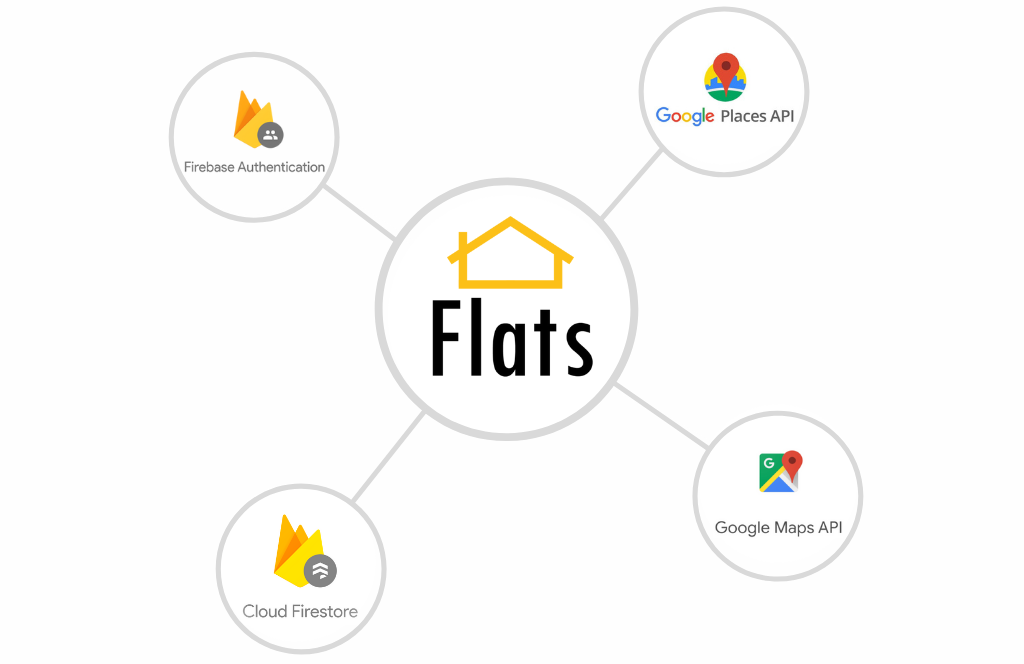
\includegraphics[scale=0.5]{images/arch.png}
            \caption{Architecture overview}
\end{figure}
        
\section{Firebase Authenticator}
We have chosen Firebase Authenticator because it provides easy-to-use backend services to authenticate users to our app.\\
We have opted for an Email and password based authentication. Once a user signs in for the first time, a new user account is created and linked to a new unique user ID that identifies the user across our app.

\section{Cloud Firestore}
We have chosen Cloud Firestore to store and retrieve all the data. Cloud Firestore is Firebase's newest database for mobile app development. It is a NoSQL, document-oriented database that means that data are stored in documents organized into collections. Unlike a SQL database, there are no tables or rows.
Each document contains a set of key-value pairs.\\
All our data are organized in 4 different collections and their structure is described here below.\\

\textbf{\textit{ChatRoom}} is the collection used for the chat service. It contains documents that are characterized by the email of the two users involved in each chat. The best way to store messages in this scenario is by using subcollections which means a collection associated with each document. In addition to this, each document has also different fields such as:
\begin{itemize}
    \item \textit{emails}: an array that contains emails of both users.
    \item \textit{lastMessage}: it contains the last message.
    \item \textit{lastMessageSendBy}: the author of the last message.
    \item \textit{lastMessageSendTs}: timestamp of the last message.\\
\end{itemize}

\textbf{\textit{Location}} is the collection used to storage data relative to each available apartment/house. Each document is associated to a single unit and it is characterized by a uniqe auto-generated ID when a unit is added by a user. Each document contains the following fields: 
\begin{itemize}
    \item \textit{description}: it contains a description of the rental ad.
    \item \textit{hostMail}: it contains the mail of the user creating the ad.
    \item \textit{location}: it contains the coordinates of the location in GeoPoint type.
    \item \textit{name}: it contains the name of the rental ad.
    \item \textit{price}: it contains the rental price.
    \item \textit{uid}: it contains the userID of the user creating the ad.
    \item \textit{urls}: it is an array containing all the urls of the image uploaded by the user.\\
\end{itemize}

\textbf{\textit{Post}} is the collection used to handle the social section. When a user creates a Post, a new document with a uniqe auto-generated ID is created as well.  Each document contains the following fields:
\begin{itemize}
    \item \textit{content}: it contains the content of the post. 
    \item \textit{flatId}: it contains the ID of the document of the location to which the post is associated. This Id is used to get the details of the apartment.
    \item \textit{title}: it contains the title of the post.
    \item \textit{uid}: it contains the userID of the user creating the post.
    \item \textit{userMail}: it contains the mail of the user creating the post.\\
\end{itemize}

\textbf{\textit{User}} is the collection containing information about each user who has a single dedicated document holding the following fields:
\begin{itemize}
    \item \textit{email}: email of the user.
    \item \textit{pic\_url}: url of the profile image of the user.
    \item \textit{username}: username of the user.\\
\end{itemize}

 We have used Cloud Firebase Storage to store and serve user-generated content, such as photos of the profile or of the rental ads.\\


\section{Google Maps API}
Considering that the visualization on the map of the geographic locations is user friendly and represents the best way to immediately identify the houses available for rent, we have opted for the Google Maps API which is a robust tool to add a custom map using Google Maps data, map displays and map gesture responses. Moreover it allows to add information on the map with customized markers. \\

\section{Google Places API}
Google Places API helps users to find points of interest and allows us to use also the Place Autocomplete service, a web service that returns place predictions in response to an HTTP request. The request specifies a textual search string and optional geographic bounds. The service can be used to provide autocomplete functionality for text-based geographic searches.
Google place APIs are not as expensive as other APIs and help users when they insert address to add a new house into the system and help us from retrieving coordinates. 

\begin{figure}[h]
    \centering
    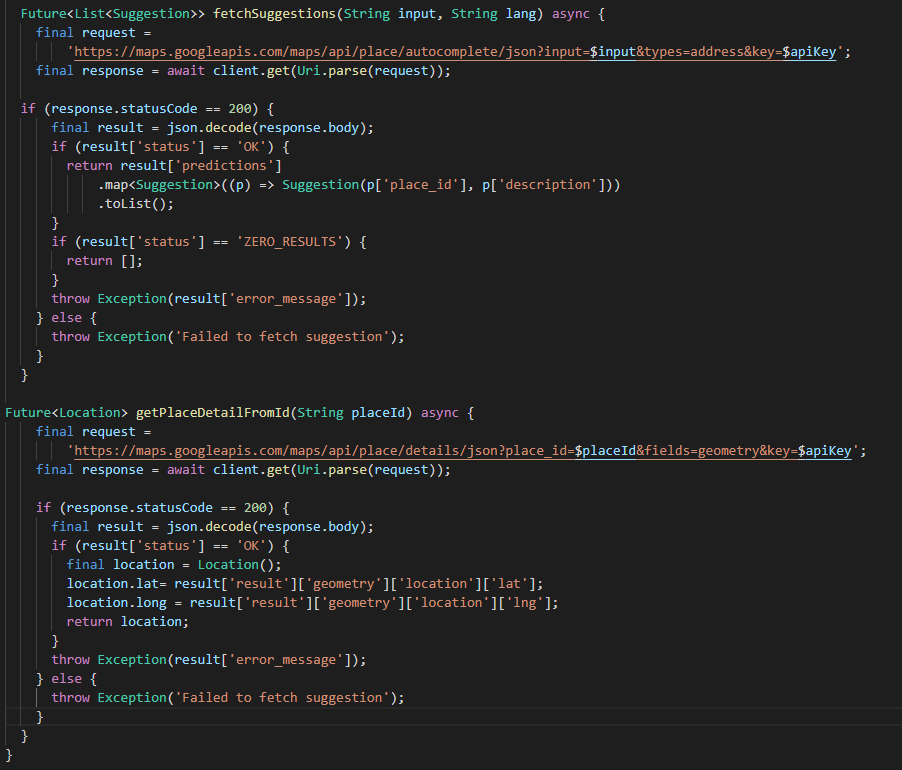
\includegraphics[width=\textwidth]{images/placesrequest.png}
    \caption{Place Autocomplete requests via Google Places API}
\end{figure}